\documentclass[10pt,a4paper]{article}
\usepackage{graphicx}
\usepackage[utf8]{inputenc}
\usepackage{amsmath}
\usepackage{amsfonts}
\usepackage{amssymb}
\author{TCP Solutions}
\title{Main project SRS}

\begin{document}

\begin{titlepage}
\begin{center}

\huge Software Requirements Specification\\[0.15cm]
\huge Forensic Medicine Mobile Application\\[0.15cm]
\large \texttt{Version: 1.0}\\[1cm]

Organization:\\
\texttt{University of Pretoria: TCP Solutions}\\[0.5cm]
GitHub:\\[0.01cm]

\begin{verbatim}
          https://github.com/CollenMphabantshi/TCP-Solutions
\end{verbatim}

Authors:\\
\texttt{Mr Mphambantshi C (10404687)\\
        Mr Legodi PT (29302732)\\
        Miss Sikhitha TP  (10346504)}\\[1cm]
        
May 22, 2014

\begin{tabular}{|l|l|l|}\hline
Name   & Date	& Changes	\\\hline
TP Solutions	& 14 May 2014	& Vision and Scope\\\hline
TP Solutions	& 15 May 2014	& Addition to vision and scope and quality requirements.\\\hline
TP Solutions	& 16 May 2014	& Software Architecture\\\hline
TP Solutions	& 23 May 2014	& Final Version\\\hline
TP Solutions	& 26 June 2014	& Functional Requirements\\\hline
TP Solutions	& 27 June 2014	& Domain Objects\\\hline
\end{tabular}

\end{center}
\end{titlepage}


\tableofcontents
\pagebreak
\section{Overview}
This document provides the overall vision and scope of the Forensic Medicine Mobile Application project. It explains and illustrates what the system will do and look like. This document basically provides the skeleton of our project. It includes the scope limitations and exclusions which will help guide the stakeholders on what is expected and not expected. This document also include use case diagram which will help explain and show the whole system.


\subsection{Document conventions}
\begin{description}
\item Documentation formulation: LaTeX
\item Unified Modelling Language: version 2.0
\end{description}

\section{Vision and Scope}


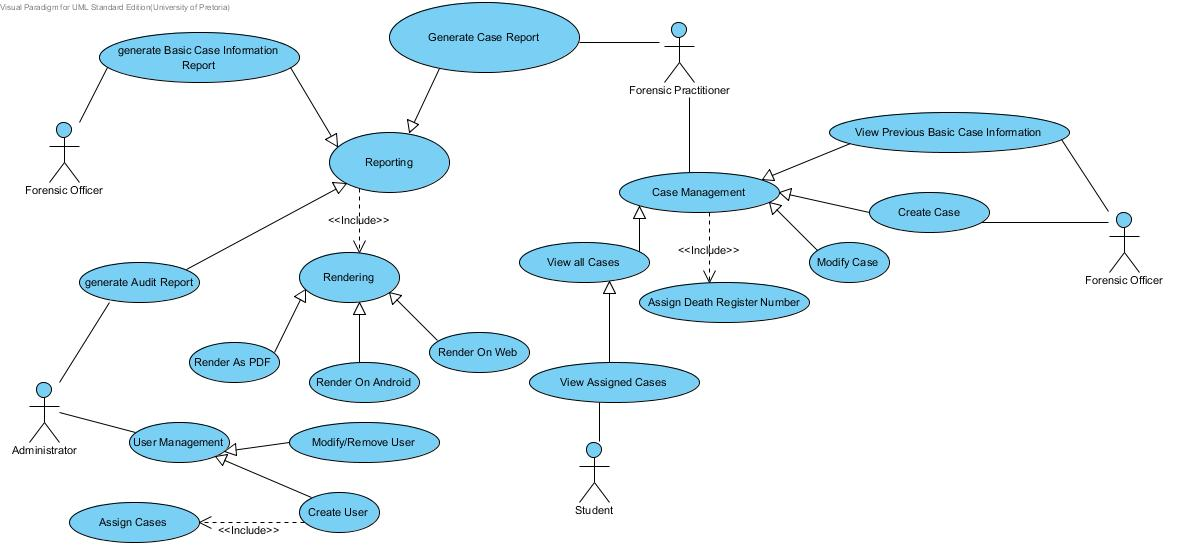
\includegraphics[scale=0.4]{DRUC.jpg}
\begin{center}

\textbf{Figure 1: The Scope of the system}
\end{center}

The proposed system is the death scene register that allow:
 \begin{itemize}
 \item Forensic officers to: 
	 \begin{itemize}
		\item Capture data from death scene – the FO’s will gather information on every scene based on the template it has on the mobile application.
		\item View basic information. The FO views personal details of the deceased and police officer who was at the scene.
	\end{itemize}
\item Forensic practitioner to:
	 \begin{itemize}
		\item Generate reports – FP’s will generate web, android and pdf reports specifically to their needs e.g. generate report of all hanging cases 2014.
		\item View all cases – every scene stored on the database they should be able to view them.
		\item Edit case information. If there was any errors made on the form such as spelling errors FPs should be able to correct them.
		\item Manage cases. FPs will dictate if the case is natural and non-natural death and do other functionalities.
	 \end{itemize}
\item Students to:
	 \begin{itemize}
		\item View all the cases cleared to them – this is for research purpose only.
	 \end{itemize}
\item Administrator to:
	 \begin{itemize}
		\item Add new users.
		\item Remove users.
		\item Edit users – change personal details and access rights.
		\item View audit report.
	 \end{itemize}
\end{itemize}

\section{Scope Limitations and Exclusions}
Pictures that demonstrate how the incident happed are excluded on this phase, maybe they can be added at a later stage.

\pagebreak
\section{Architecture requirements}
\subsection{Access channel requirements}
\indent It is going to be accessed by humans using android and web application.
                                                                                               
\subsection{Quality requirements}
\begin{itemize}
\item\textbf{Performace}
\begin{itemize}
	\item The system should process all the reports within 10 seconds.
	\item It should send the information to the server within seconds.
\end{itemize}
               
\item\textbf{Reliability}
  \begin{itemize}
  	\item The system should be up and running all the time.
  	\item Easy and fast access to the database.
  \end{itemize}
\item\textbf{Scalability}
\begin{itemize}
  	\item The system should be able to handle all death scenes captured information.
  	\item It should allow additional templates.
  \end{itemize}
\item\textbf{Security}
\begin{itemize}
  	\item The system is accessible to users who are authorized.
  	\item System users will have different permission.
  	\item Information about death scenes will be encrypted.
  	\item Information stored by forensic officers will not be edited after the submission.
  \end{itemize}
\item\textbf{Flexibility} 
\begin{itemize}
  	\item If something happen when the forensic officer is capturing information, it should automatically be stored in the server.
  \end{itemize}
\item\textbf{Maintanability}					
 \begin{itemize}
   	\item The system will be maintained every time the client needs new changes.
   \end{itemize}        
\item\textbf{Auditability}         
      \begin{itemize}
        	\item The system should record all the changes made to the data stored, by showing whom, when and what was changed.
        	\item It will also show old and new values.
        	
        \end{itemize} 
\item\textbf{Usability}
\begin{itemize}
     \item Users should be able to use the system without prior
      training.                                                       \item The system will be in English.   
 \end{itemize}
 
\end{itemize}

\subsection{Integration requirements}
\begin{itemize} 
\item Database will be created from scratch.
\item The android application will be connected to the web service and the web service connected to the server.
\end{itemize}
   
\subsection{Architecture constraint}                       
\begin{itemize}
\item The device that will be used is Asus nexus 7
\item Android SDK
\item MySQL
\item HTML5,PHP,apache(Afrihost)
\item Java, JavaScript
\item Ajax, jQuery
\item The mobile client must be running on an android application.
\end{itemize}
\pagebreak

\section{Software Architecture Documentation}
\subsection{Architecture requirements}
\begin{enumerate}
\item Architectural scope
\begin{description}
\item The database will run on Afrihost
\begin{center}
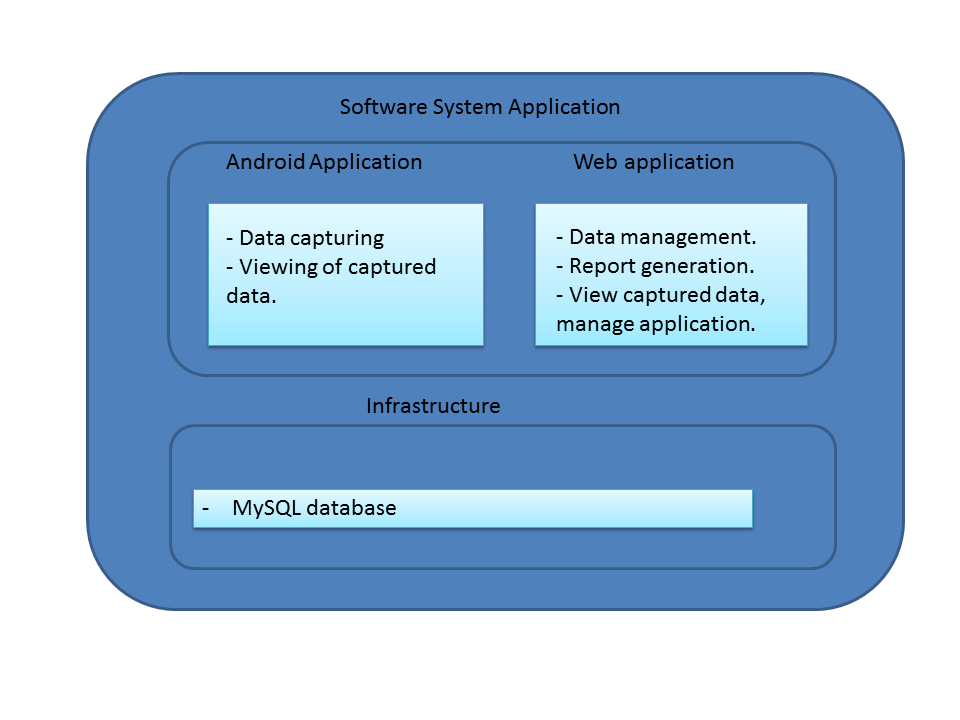
\includegraphics[scale=0.4]{Architecture-scope.png}
\textbf{Figure 2:Architectural Scope}
\end{center}
\item [Android app]

\begin{itemize}
\item The android application will be used to capture information on death scenes.
\item View information based on clearance.
\end{itemize}

\item [Web app]

\begin{itemize}
\item will be used for data management.
\item Report generation.
\item System administration.
\end{itemize}

\item [Infrastructure]

\begin{itemize}
\item Data storage, MySQL database on Afrihost.
\end{itemize}

\end{description}


\item Quality requirements

\begin{description}
\item [Security]

\begin{itemize}
\item Only authorised people should be able to have access to the system.
\item Only administrator should register people.
\end{itemize}

\item [Auditability]

\begin{itemize}
\item Any change made to data stored should be recorded.
\item Record what, who and when changes were made.
\end{itemize}

\item [Performance]

\begin{itemize}
\item Data should be sent in real time e.g. from forensic officer to forensic practitioner should receive it within 10 seconds.
\end{itemize}

\item [Reliability]

\begin{itemize}
\item The server should run all the time (24/7 - 365) and the connection should always be active.
\item Only administrator should register users.
\end{itemize}

\item [Usability]

\begin{itemize}
\item All the users should be able to use the system without any prior training.
\end{itemize}

\end{description}

\item Integration and Access channel
\begin{description}
\item [Access Channel]

\begin{itemize}
\item Accessible by humans through the following channels:	Admin – the access it through web application and FO, FP and students – they show access the system through mobile application.
\end{itemize}

\item [Integration Channel]

\begin{itemize}
\item The new SQL database will be created in Afrihost.
\end{itemize}
\end{description}

\item Architectural constraints
\begin{description}
\item [The system will use the following constraints]

\begin{itemize}
\item Android SDK
\item REST web services
\item The system will be deployed in Asus Nexus 7 OS Android 4.1 jelly bean.
\end{itemize}

\item [Technologies to be used]

\begin{itemize}
\item Java, PHP, HTML, JavaScript, MySQL,  JQuery, CSS
\end{itemize}
\end{description}

\end{enumerate}
\subsection{Architectural Pattern}


\begin{center}
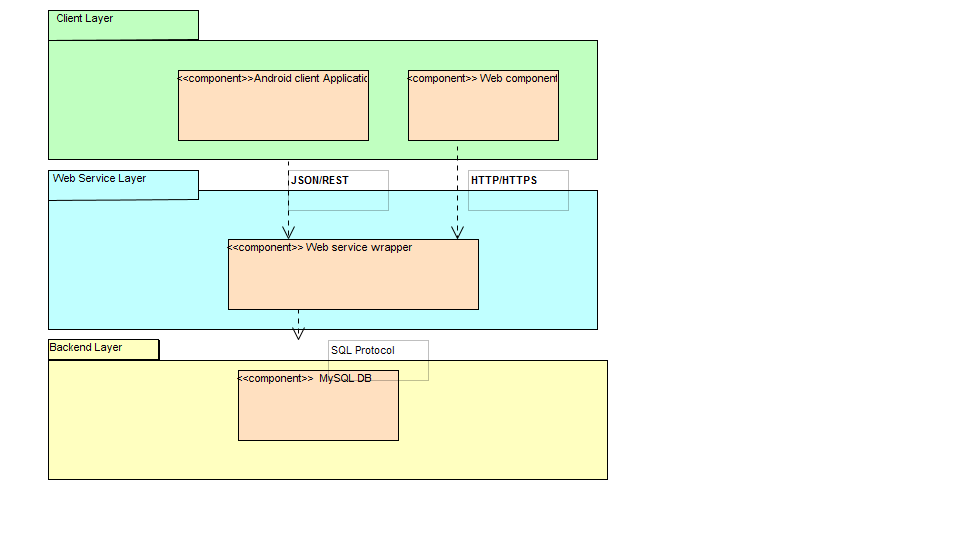
\includegraphics[scale=0.4]{Architectural-Pattern.png}

\textbf{Figure 3: Architectural layered pattern}
\end{center}

\begin{description}
\item [The Architectural pattern]

\begin{itemize}
\item Provides access to humans  - Client
\item Provides Functionality  and objects required to client layer -> Web service
\item Host database - Backend layer
\end{itemize}

\item [The communication protocol are also shown. They include]

\begin{itemize}
\item HTTP/HTTPS from the browser to the web module.
\item Provides Functionality  and objects required to client layer - Web service
\item JSON/REST/HTTP/HTTPS for the web services between the Android application and the database.
\end{itemize}

\end{description}

\subsection{Use of reference architectures and frameworks}

\begin{center}
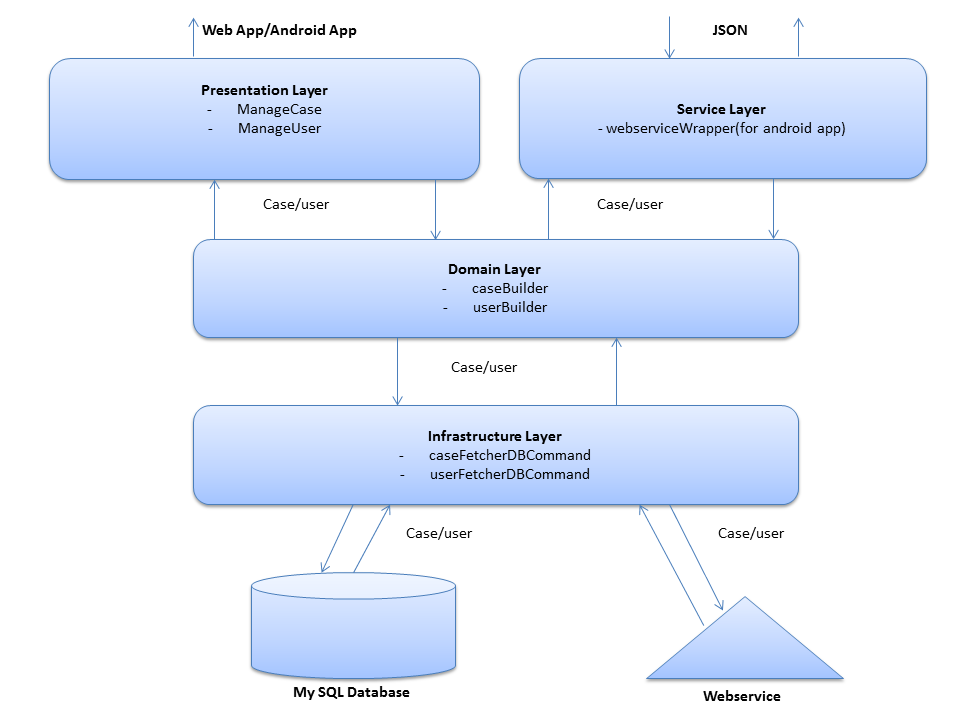
\includegraphics[scale=0.4]{Framework.png}
\textbf{Figure 4: Three Layer Architecture}
\end{center}


\begin{description}
\item [Presentation Layer]

\begin{itemize}
\item This User interface Layer. The UI is responsible for creating and displaying the user interface and handling user interaction. It’s going to be in Android App and Web App. It gets data from Domain layer.
\end{itemize}

\item [Service Layer]

\begin{itemize}
\item This is the Web Service Layer. Responsible for showing web service API and returning method results as JSON. It gets data from Domain Layer.
\end{itemize}

\item [Domain Layer]

\begin{itemize}
\item This is the Business logic, it is responsible for business logic of the application. All functions and objects used are going to be modelled here. It gets data from Infrastructure layer.
\end{itemize}

\item [Infrastructure Layer]

\begin{itemize}
\item It responsible for querying database, calling web service and send emails.
\end{itemize}
\end{description}


\section{Functional Requirements}
\subsection{Introduction}


\subsection{Required functionality}
\begin{enumerate}
	\item User Management functionality
	\begin{center}
		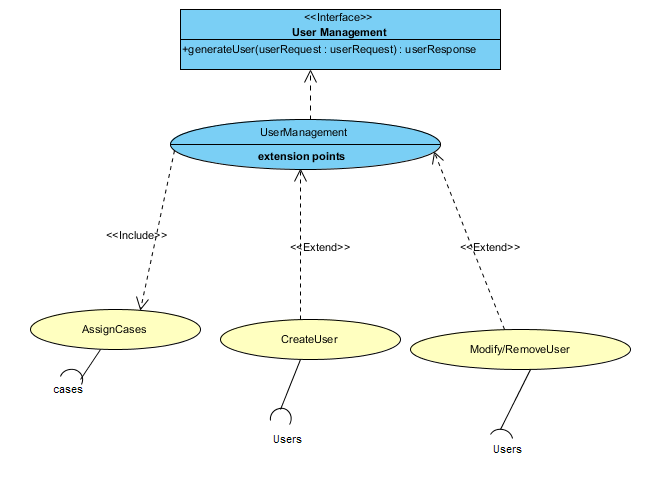
\includegraphics[scale=0.4]{UserManagementRequirementFunctionality.png}
		
		\textbf{Figure 5: User Management Use Case}
	\end{center}
	\begin{itemize}
		\item The user management functionality allows the administrator to assign cases to students.
		\item Allows the administrator to add new users.
		\item Allows the administrator to modify user information.
		\item Allows the administrator to remove users.
	\end{itemize}
	\item Case Management functionality
	\begin{center}
		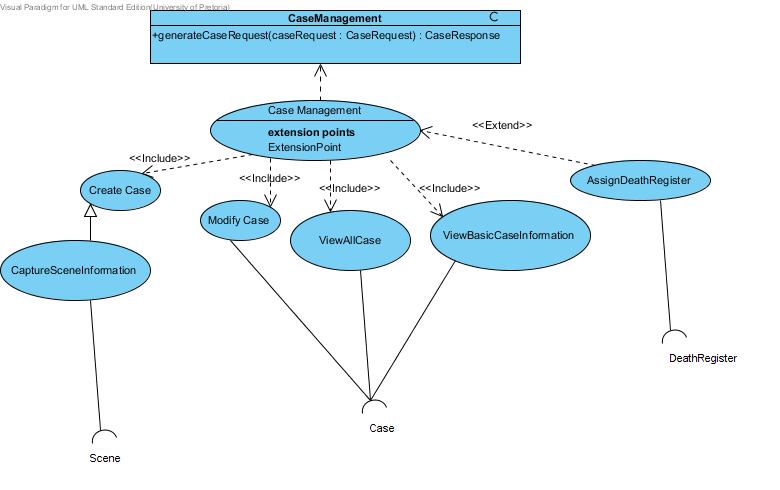
\includegraphics[scale=0.4]{CaseManagementUseCase.png}
		
		\textbf{Figure 6: Case Management Use Case}
	\end{center}
	\begin{itemize}
		\item The case management functionality allows the Forensic Officers to create new cases.
		\item Allows the Forensic Officers to view basic information of the case they created after submission.
		\item Allows the Forensic Practitioner to modify/add additional information on the case.
		\item Allows the Forensic Practitioner to view all cases.
		\item Allows the Forensic Practitioner to assign a death register to non-natural cases.
		\item Allows Masters and Honours students to view all cases they are assigned to.
	\end{itemize}
	\item Reporting functionality
		\begin{center}
			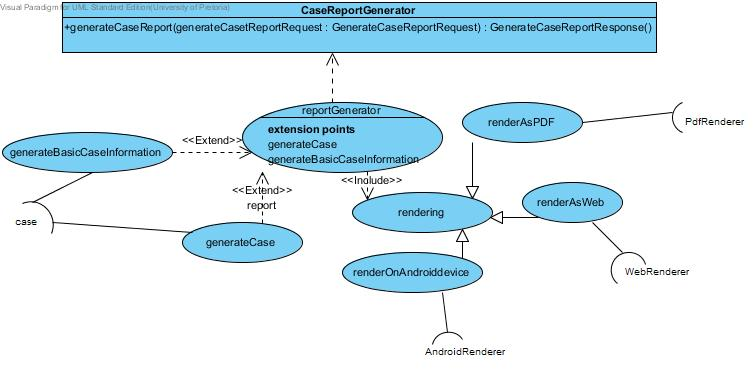
\includegraphics[scale=0.4]{caseGeneratorReport.jpg}
			
			\textbf{Figure 7: Case Report Generator Use Case}
		\end{center}
		\begin{itemize}
			\item The reporting functionality allows different users to generate reports about cases, users and audit logs.
			\item It allows users to generate a report rendered on the web.
			\item It allows users to generate a report rendered on the android device.
			\item It allows users to generate a report rendered to pdf file.
		\end{itemize}
	\item Domain Objects
	\begin{enumerate}
		\item Overview
		\begin{description}
			\item The main domain objects are
		
			\item Persons – This may be assigned forensic officers, forensic practitioner, administrator and students with respect to different responsibilities and access level.
			\item Cases - it can be aggregated into different type of scenes and different type of cases (e.g. natural and un-natural)
			
		\end{description}
		\begin{center}
			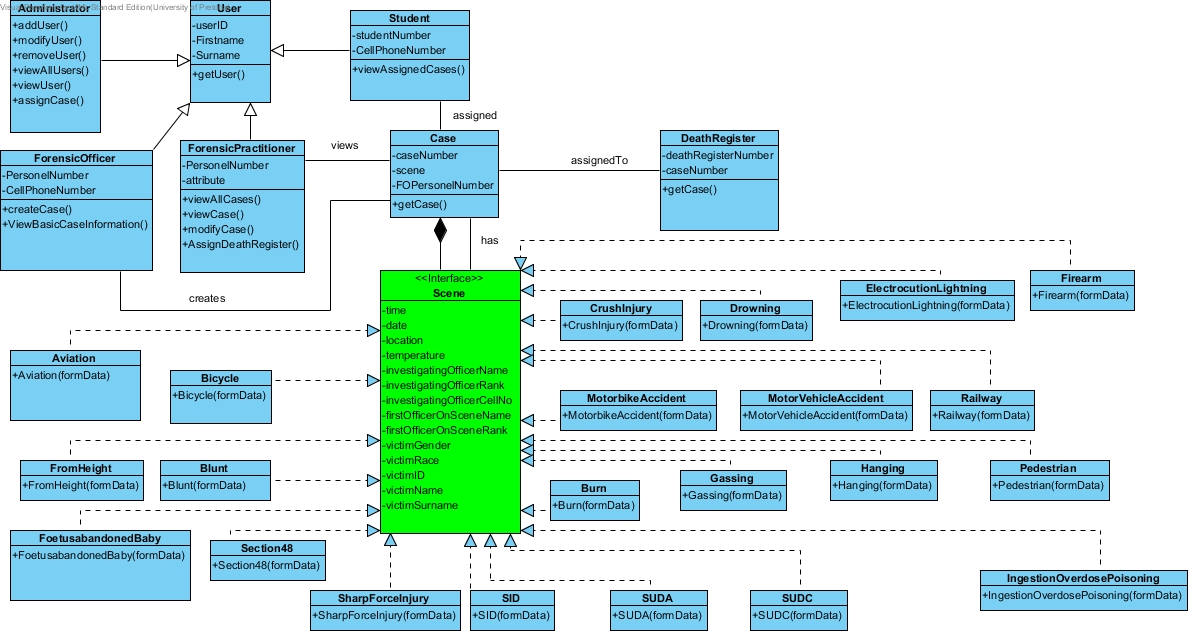
\includegraphics[scale=0.4]{ClassDiagram1.jpg}
			
			\textbf{Figure 8: Overview of data structures and relationships for the core domain objects}
		\end{center}
		
		\item Users
		\begin{description}
			\item All users are going to be registered in the database and authentication will be done against the database.
			\item The registered user’s information will include the name, surname, portfolio and its details, roles and responsibility, personnel ID and access rights.
			\item The user class will be identified by a unique role of a user.
			\item The administrator will be able to add, remove and edit the users in the system. Every change that is made will be recorded in the audit log. The administrator should also be able to assign cases to user in the system e.g. assign 50 students to a hanging case for research. 
		\end{description}
		\item Cases
		\begin{description}
			\item Cases can be either natural or un-natural. Forensic officer can decide whether the case is natural or un-natural. And for unnatural case, every case will be assigned a different death registry and will be stored in a special registry of un-natural cases.
			\item Every case has a scene and scenes are divided as follows:
			\begin{itemize}
				\item Sudden and unexpected death
					\begin{itemize}
						\item Sudden unexpected death of an infant (SUDI)
						\item Sudden unexpected death of a child  (1 – 18 years)
						\item Sudden unexpected death of an adult/found dead
					\end{itemize}
				\item Foetus / Abandoned baby
				\item Section 48  death –surgical case
				\item Road traffic accidents
					\begin{itemize}
						\item Pedestrian vehicle accident
						\item Bicycle accident
						\item Motorbike accident
						\item Motor vehicle accident
					\end{itemize}
				\item Railway accident
				\item Aviation accident
				\item Fall/push/jump from height
				\item Crush injury
				\item Firearm discharge/gunshot wound
				\item Sharp force injury/stab injury
				\item Blunt force injury/assault
				\item Drowning
				\item Gassing
				\item Hanging
				\item Ingestion/overdose/poisoning
				\item Burns
				\item Lightning/electrocution
			\end{itemize}
		\end{description}
	\end{enumerate}
\end{enumerate}



\subsection{Use case prioritization}
\begin{enumerate}
	\item Login(critical)
		All the system functionality should be accessible by users who are logged in.
	\item Case management(critical)
		The system should be able to create a case, modify, view and assign a death register number; because this are the core functionalities of the system. 
	\item User management(important )
		The system must be able to allow only specific users to view specific information, this will ensure that the system is secured and privacy is maintained.
	\item Reporting
		It will be useful for accountability and auditability.
\end{enumerate}  

\subsection{Use case/Services contracts}

   \begin{center}
   	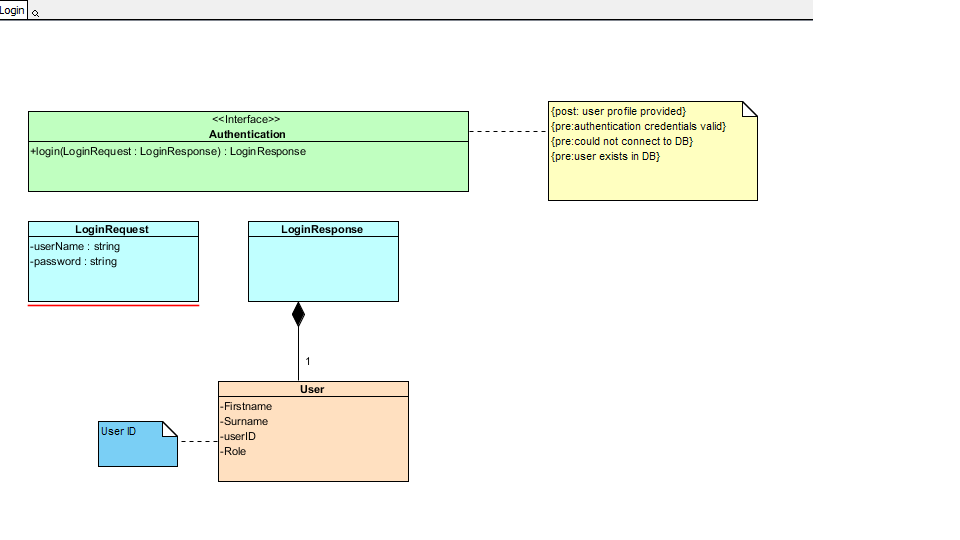
\includegraphics[scale=0.4]{LoginServiceContract.png}
   	
   	\textbf{Figure 9: Login Service Contract}
   \end{center}
\subsection{Process Specification}
\begin{center}
	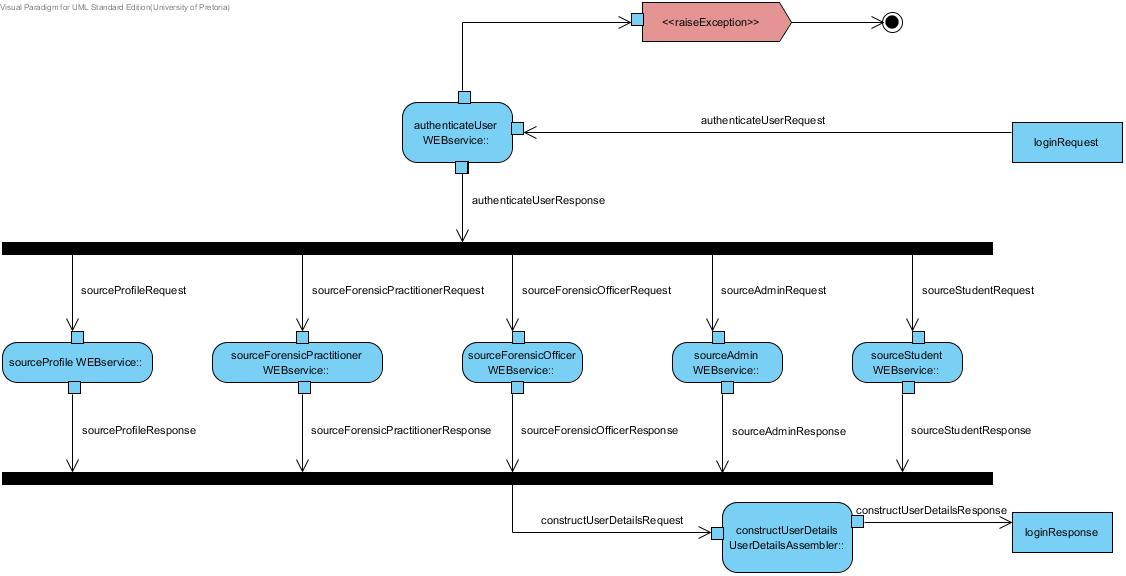
\includegraphics[scale=0.4]{loginActivity.jpg}
	\textbf{Figure 10: Login Activity Diagram}
\end{center}
\pagebreak

\section{Open Issues}

\section{Glossary}
\begin{description}
	\item [Forensic officer (FO)] – a specially trained crime scene officer that collects the finding evidence that will be analyzed back at the lab by forensic scientist or forensic practitioner. 
	\item [Forensic practitioner (FP)] - also referred to as crime scene investigators and forensic science technicians examine pieces of evidence to provide crucial support in criminal investigations. Their professional expertise is sought in laboratories, crime scenes and courtrooms.
	\item [Stakeholders] - is anybody who can affect or is affected by an organization, strategy or project. They can be internal or external and they can be at senior or junior levels.
	\item [Students] – honors and masters students who are doing research as part of their studies.
	\item[MySQL] MySQL (Structured Query Language) is an open-source relational database management system.
	
	\item[PDF] Portable Document Format is a file format for capturing and sending electronic documents in exactly the intended format.
	\item[UML] Unified Modelling Language is a general-purpose modelling language in the field of software engineering. It provides a set of graphic notation techniques to create visual models of object-oriented software-intensive systems. 
	

\end{description}

\end{document}
